% !TEX root = main.tex
\documentclass[a4paper, UKenglish, 11pt]{uiomaster}
\usepackage{lipsum}
\usepackage[subpreambles=true]{standalone}
\usepackage{graphicx}


\begin{document}

\chapter{Creating EEG Data}
In preparation for the application of neural networks to address inverse problems, the acquisition of a substantial and appropriate EEG dataset is essential. This chapter focuses on utilizing the New York Head model (NYHM) in conjunction with the current dipole approximation to construct biophysically realistic EEG data.

\section{Simulation of EEG Signals from single dipoles}
\rednote{include range of x, y, z values !! and maybe eeg ? }
The New York Head model (NYHM) is integrated into the Python module LFPy. Within LFPy, we use the \emph{NYHeadModel} class to calculate EEG signals originating from a current dipole moment $\textbf{P}$. The current dipole moments of the LFPy kit are expressed in terms of nA$\mu$m, while the EEG signals derived from the NYHM are recomputed into units of mV. For more information about the LFPy package, we refer the reader to \url{https://lfpy.readthedocs.io/en/latest/readme.html#summary}.

The cortical matrix of the NYHM comprises 74,382 discrete points, each corresponding to a possible location for localizing dipole sources. In the context of simulating EEG measurements, the procedure commences with the random selection of positions from these points to serve as the locations for placing dipoles. Each simulated EEG sample entails a solitary dipole positioned at one of the randomly chosen locations. As the primary objective is to address the inverse problem, maintain uniform amplitudes for the dipole signals, as their variation is not of primary concern. By setting these amplitudes to $10^7$ nA $\mu$m, the resulting EEG measurements span a range of approximately -1 to 1 $\mu$V.

To ensure that the dipole orientations are predominantly aligned with the depth direction of the cortex, we assign dipole strengths solely in the z-direction. Moreover, a rotation procedure is employed for each dipole moment, orienting it perpendicular to the cerebral cortex. Occasionally, this orientation results in a dipole moment pointing outward, toward an EEG electrode. Alternatively, due to the convoluted structure of the cortex, the dipole moment may be directed back into the cortex, eventually aligning with an EEG electrode after traversing a greater distance. This phenomenon arises from the complex folding patterns of the human cortex, where the EEG signal contribution of a dipole moment depends on its position within a sulcus or gyrus \cite{naess2021biophysically}.

The New York Head model (NYHM) generates EEG signals as time series data, reflecting the structure of real-world measurements. As a result, the inherent format of EEG data deviates from a one-dimensional representation, instead adopting a matrix configuration of 231x1601 dimensions. In this arrangement, 231 values represent measurements from scalp recording electrodes, with 1601 time steps marking the temporal progression. However, as mentioned in the preceding chapter, EEG analysis often centers on specific frequency components within each temporal instance of measurement. This practice effectively reduces the multidimensional EEG data and eliminates less relevant recordings.

In the context of our analysis, which aims to pinpoint sources of neural activity, the transition to one-dimensional data proves to be benefitial. This transition contributes to problem simplification and computational efficiency. Importantly, our approach diverges from the conventional practice of extracting diverse frequency spectra to identify anomalous activity. Instead, we leverage the initial time step of the EEG recording to encapsulate epileptiform behavior of interest. This method works well because there are no confusing signals from brain activity or unclear background noise in the simulated data. This makes the analysis very reliable and solid. Our focus is directed towards the signal at $t = 1$, corresponding to the first time step of the recording. As a result, our methodology yields a one-dimensional EEG signal, effectively encapsulating insights into the spatial distribution of EEG patterns and the interrelation between these patterns and the specific locations of dipole sources within the cerebral cortex.

\rednote{Should we show a single sample will look like?}



\section{The Effect of dipole location and orientation}
According to Naess et al. (2021) \cite{naess2021biophysically}, EEG signals are not particularly sensitive to minor shifts in the precise location of neural current dipoles. This insensitivity can be explained by the fact that relative to the dimensions of individual neurons and the thickness of the human cortex, EEG electrodes are located far away from cortical neural sources. Given the substantial spatial smearing and the considerable distance between EEG electrodes and cortical sources, millimeter-scale shifts in the positions of neural current dipoles tend to have a limited impact on the EEG signal. This is further illustrated in Figure \ref{fig:neighbour_dipoles}, where we present three EEG signals corresponding to dipoles situated at neighboring points within the NYHM cortical matrix.

The plotted EEG signals of the blue and green dipoles in Figure \ref{fig:neighbour_dipoles} exhibit a considerable overlap. This overlapping pattern is supported by a high correlation coefficient of 0.966, indicating a robust positive relationship between these measurements. In simpler terms, as one variable increases, the other variable increases proportionally - an observation evident from the figure. In contrast, the EEG signals of the blue and red dipoles exhibit less resemblance. The correlation coefficient between these signals is 0.695, denoting a somewhat smaller linear relationship. Importantly, the observed differences can be attributed to the shifts in the normal vector of the red dipole. This shift is also evident for the normal vectors of the blue and green dipole, but is more evident considering the red dipole. When choosing neighboring dipoles in the terms of distance within the NYHM, shifts in the normal vectors also arises due to the rotation procedure used during data generation to ensure dipole orientations are perpendicular to the cerebral cortex. Due to the complex folding of the cortex, shifts in the dipole's location will often lead to corresponding shifts in normal vectors as well. As a result, distinct differences emerge in the corresponding EEG signal.

%Despite the common belief that neurons in the upper cortical layers would dominate the EEG due to their proximity to the electrode compared to neurons in deeper layers, such location differences do not significantly affect the EEG signals. This phenomenon can be explained by the fact that the low conductivity of the skull introduces a spatial low-pass filtering effect, which mitigates the impact of location discrepancies.
% Maybe what is meant here is that we therefore only consider the outer corical surface

\begin{figure}[!htb]
    \centering
    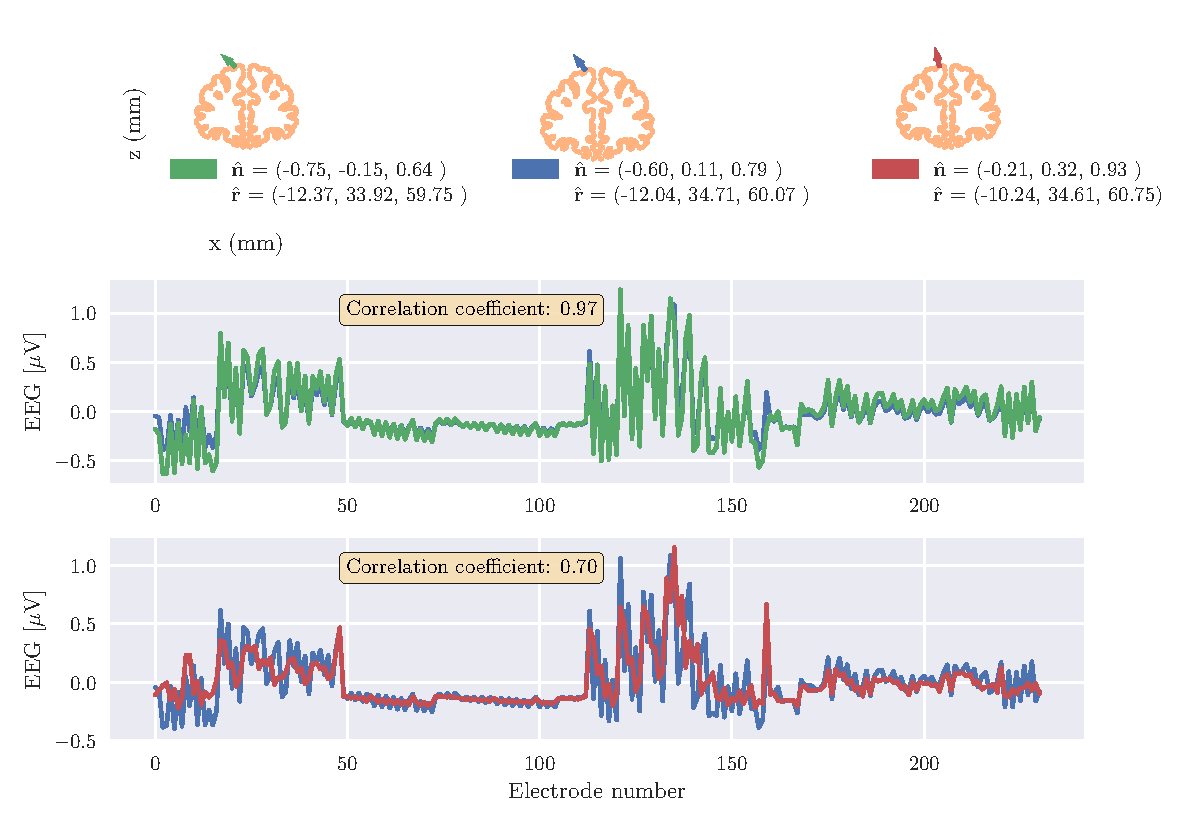
\includegraphics[width=\linewidth]{figures/compare_dipoles.pdf}
    \caption{EEG signals plotted against electrode number for three neighbouring dipoles with normal vectors (-0.60, 0.11, 0.79), (-0.75, -0.15, 0.64), (-0.21, 0.32, 0.93) and positions (-12.04, 34.71, 60.07), (-12.37, 33.92, 59.75), (-10.24, 34.61, 60.75). The correlation coefficient between the blue and green dipole is 0.97, while it is 0.70 for the blue and red dipole.}
    \label{fig:neighbour_dipoles}
\end{figure}

To further illustrate this, consider the effect of dipole orientation on EEG outcomes. Figure \ref{fig:gyrus_and_sulcus_EEG}, borrowed from work done by Tornjørn Ness and Gaute Einevoll, represent the EEG signals obtained from two manually selected dipole locations within the New York head model. These dipoles are situated in a gyrus and a sulcus, respectively, and exhibit distinct EEG patterns. In general, the contribution of an individual current dipole to the EEG signal is maximized the dipole is perpendicularly situated within a gyrus, as depicted in Figure \ref{fig:gyrus_and_sulcus_EEG}B. Contrastingly, when a dipole is placed in a sulcus with a perpendicular orientation, a significant EEG contribution may still be observed, however unlike the dipole in the gyrus, it exhibits a more dipolar pattern, as shown in Figure \ref{fig:gyrus_and_sulcus_EEG}C.


\begin{figure}[!htb]
    \centering
    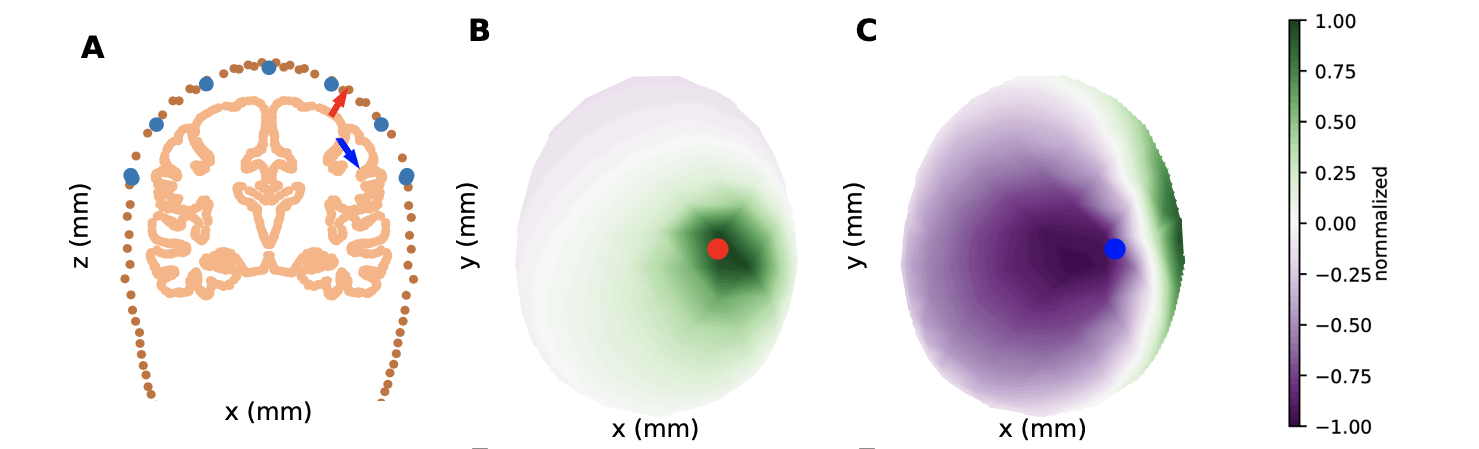
\includegraphics[width=\linewidth]{figures/gyrus_and_sulcus_EEG.png}
    \caption{A: Two selected dipole locations in the New York head model: one in a gyrus (red) and one in a sulcus (blue). The head model is viewed from the side (x, z-plane). Close to the chosen cross-section plane, EEG electrode locations are marked in light blue. Available dipole locations near the cortical cross-section form an outline of the cortical sheet and are marked in pink. The current dipole moment for all cases was $10^7$ nA$\mu$m. B: Interpolated color plot of EEG signal from the gyrus dipole, viewed from the top (x, y-plane). The plotted EEG signal is scaled, with a maximum value of 1.1 $\mu$V. C: Interpolated color plot of EEG signal from the sulcus dipole. The plotted EEG signal is scaled, with a maximum value of 0.7 $\mu$V. This Figure is borrowed from work done by Torbjørn Ness and Gaute Einevoll \cite{naess2021biophysically}.}
    \label{fig:gyrus_and_sulcus_EEG}
\end{figure}

Further exploration of dipole orientation's impact is presented in Figure \ref{fig:dipole_orientation}. This figure is borrowed from work done by Torbjørn Ness and Gaute Einevoll. Here, we observe EEG signals from identical dipoles positioned in various folding patterns of the cortical surface. These patterns reveal that the orientation of the current dipole moment significantly influences the EEG outcome. Firstly, Figure \ref{fig:dipole_orientation}A and \ref{fig:dipole_orientation}C provide an expanded illustration of the aforementioned scenarios, incorporating additional dipole moments located in a gyrus and a sulcus, respectively. In Figure \ref{fig:dipole_orientation}B, where a collection of dipoles points randomly upwards and downwards, the EEG signal contribution appears to diminish significantly. Conversely, when the dipoles align in the depth direction of the cortex and are distributed across both gyrus and sulcus, we can expect an EEG contribution in between what we saw from Figure \ref{fig:dipole_orientation}A and \ref{fig:dipole_orientation}B, as depicted in Figure \ref{fig:dipole_orientation}D. Lastly, Figure \ref{fig:dipole_orientation}E demonstrates the minimal EEG contribution observed when the dipoles are divided between two opposing sulci.


\begin{figure}[!htb]
    \centering
    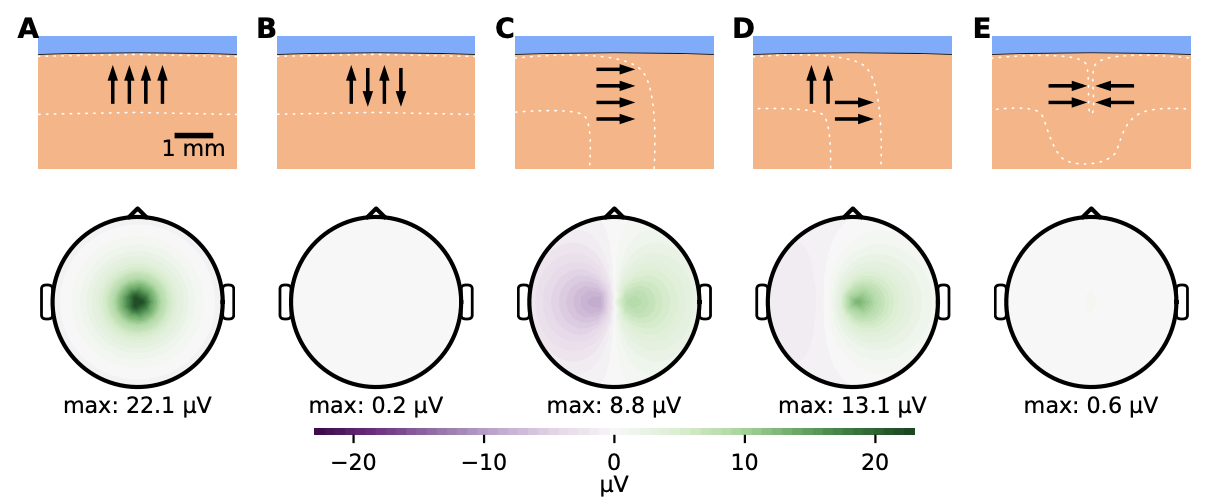
\includegraphics[width=\linewidth]{figures/dipole_orientation.png}
    \caption{Different folding patterns of the cortical surface are represented by white dashed lines. EEG signals are calculated from four identical current dipoles with varying orientations. A: Dipoles aligned in the same direction within a gyrus. B: Dipoles pointing in opposite directions within a gyrus. C: Dipoles aligned in the same direction within a sulcus. D: Dipoles distributed between a gyrus and a sulcus, pointing towards the cortical surface. E: Dipoles divided between opposing sulci, pointing towards the cortical surface.
    Each panel features a dipole moment magnitude of 10 nAm, and the dipoles are positioned at the centers of the arrows in the top row. This Figure is borrowed from work done by Torbjørn Ness and Gaute Einevoll \cite{naess2021biophysically}.}
    \label{fig:dipole_orientation}
\end{figure}

% This is not the case for a simple dipole moment, but might be an issue when giving the populations a radii
% In our analysis, we simplify the scenario by considering one current dipole at a time, which allows us to avoid cancellations of potentials and obtain simpler EEG potentials. While this simplification may not capture the full complexity of neural activity, it provides us with a clearer understanding of the relationship between dipole orientation and EEG signals.



\section{Noise}
Experimental EEG recordings inevitably contain noise, which can interfere with the accurate analysis of brain activity. Artifacts, which are signals recorded by EEG but originating from sources other than the human brain, pose a particular challenge. Some artifacts can mimic genuine epileptiform abnormalities or seizures, underscoring the importance of identifying and distinguishing them from true brain waves \cite{sazgar2019eeg}.

Artifacts can be classified into two categories based on their origin. Physiological artifacts arise from the patient's own physiological processes, including ocular activity, muscle activity, cardiac activity, perspiration, and respiration. Technical artifacts, on the other hand, originate from external factors such as cable and body movements or electromagnetic interferences \cite{bitbrain}.

Filtering techniques are commonly employed to remove artifacts from EEG recordings prior to analysis. However, in the case of simulated EEG data, the need for artifact removal is eliminated as the data inherently lacks noise. Simulated EEG data can be considered as pre-filtered and preprocessed, ensuring a high signal-to-noise ratio (SNR) \cite{wiki-snr}. Nevertheless, to avoid overfitting and account for technical considerations, it is necessary to introduce noise to the data before feeding it into the neural network. This introduction of the noise is vital in order to make the trained neural network more likely to accurately handle real EEG recordings.

In our approach, we recognize that the introduction of noise to the simulated EEG data is an essential step to enhance the robustness of the trained neural network and ensure its ability to handle real EEG recordings effectively. Although the specific characteristics and quantity of noise have not been the primary focus of our study, we have opted for a straightforward approach. Our final dataset incorporates normally distributed noise with a mean of 0 and a standard deviation equal to 10$\%$ of the standard deviation observed in the simulated EEG recordings. By introducing this noise, we introduce random variations around each data point while preserving the overall normalization properties of the dataset.

\begin{figure}[!htb]
    \centering
    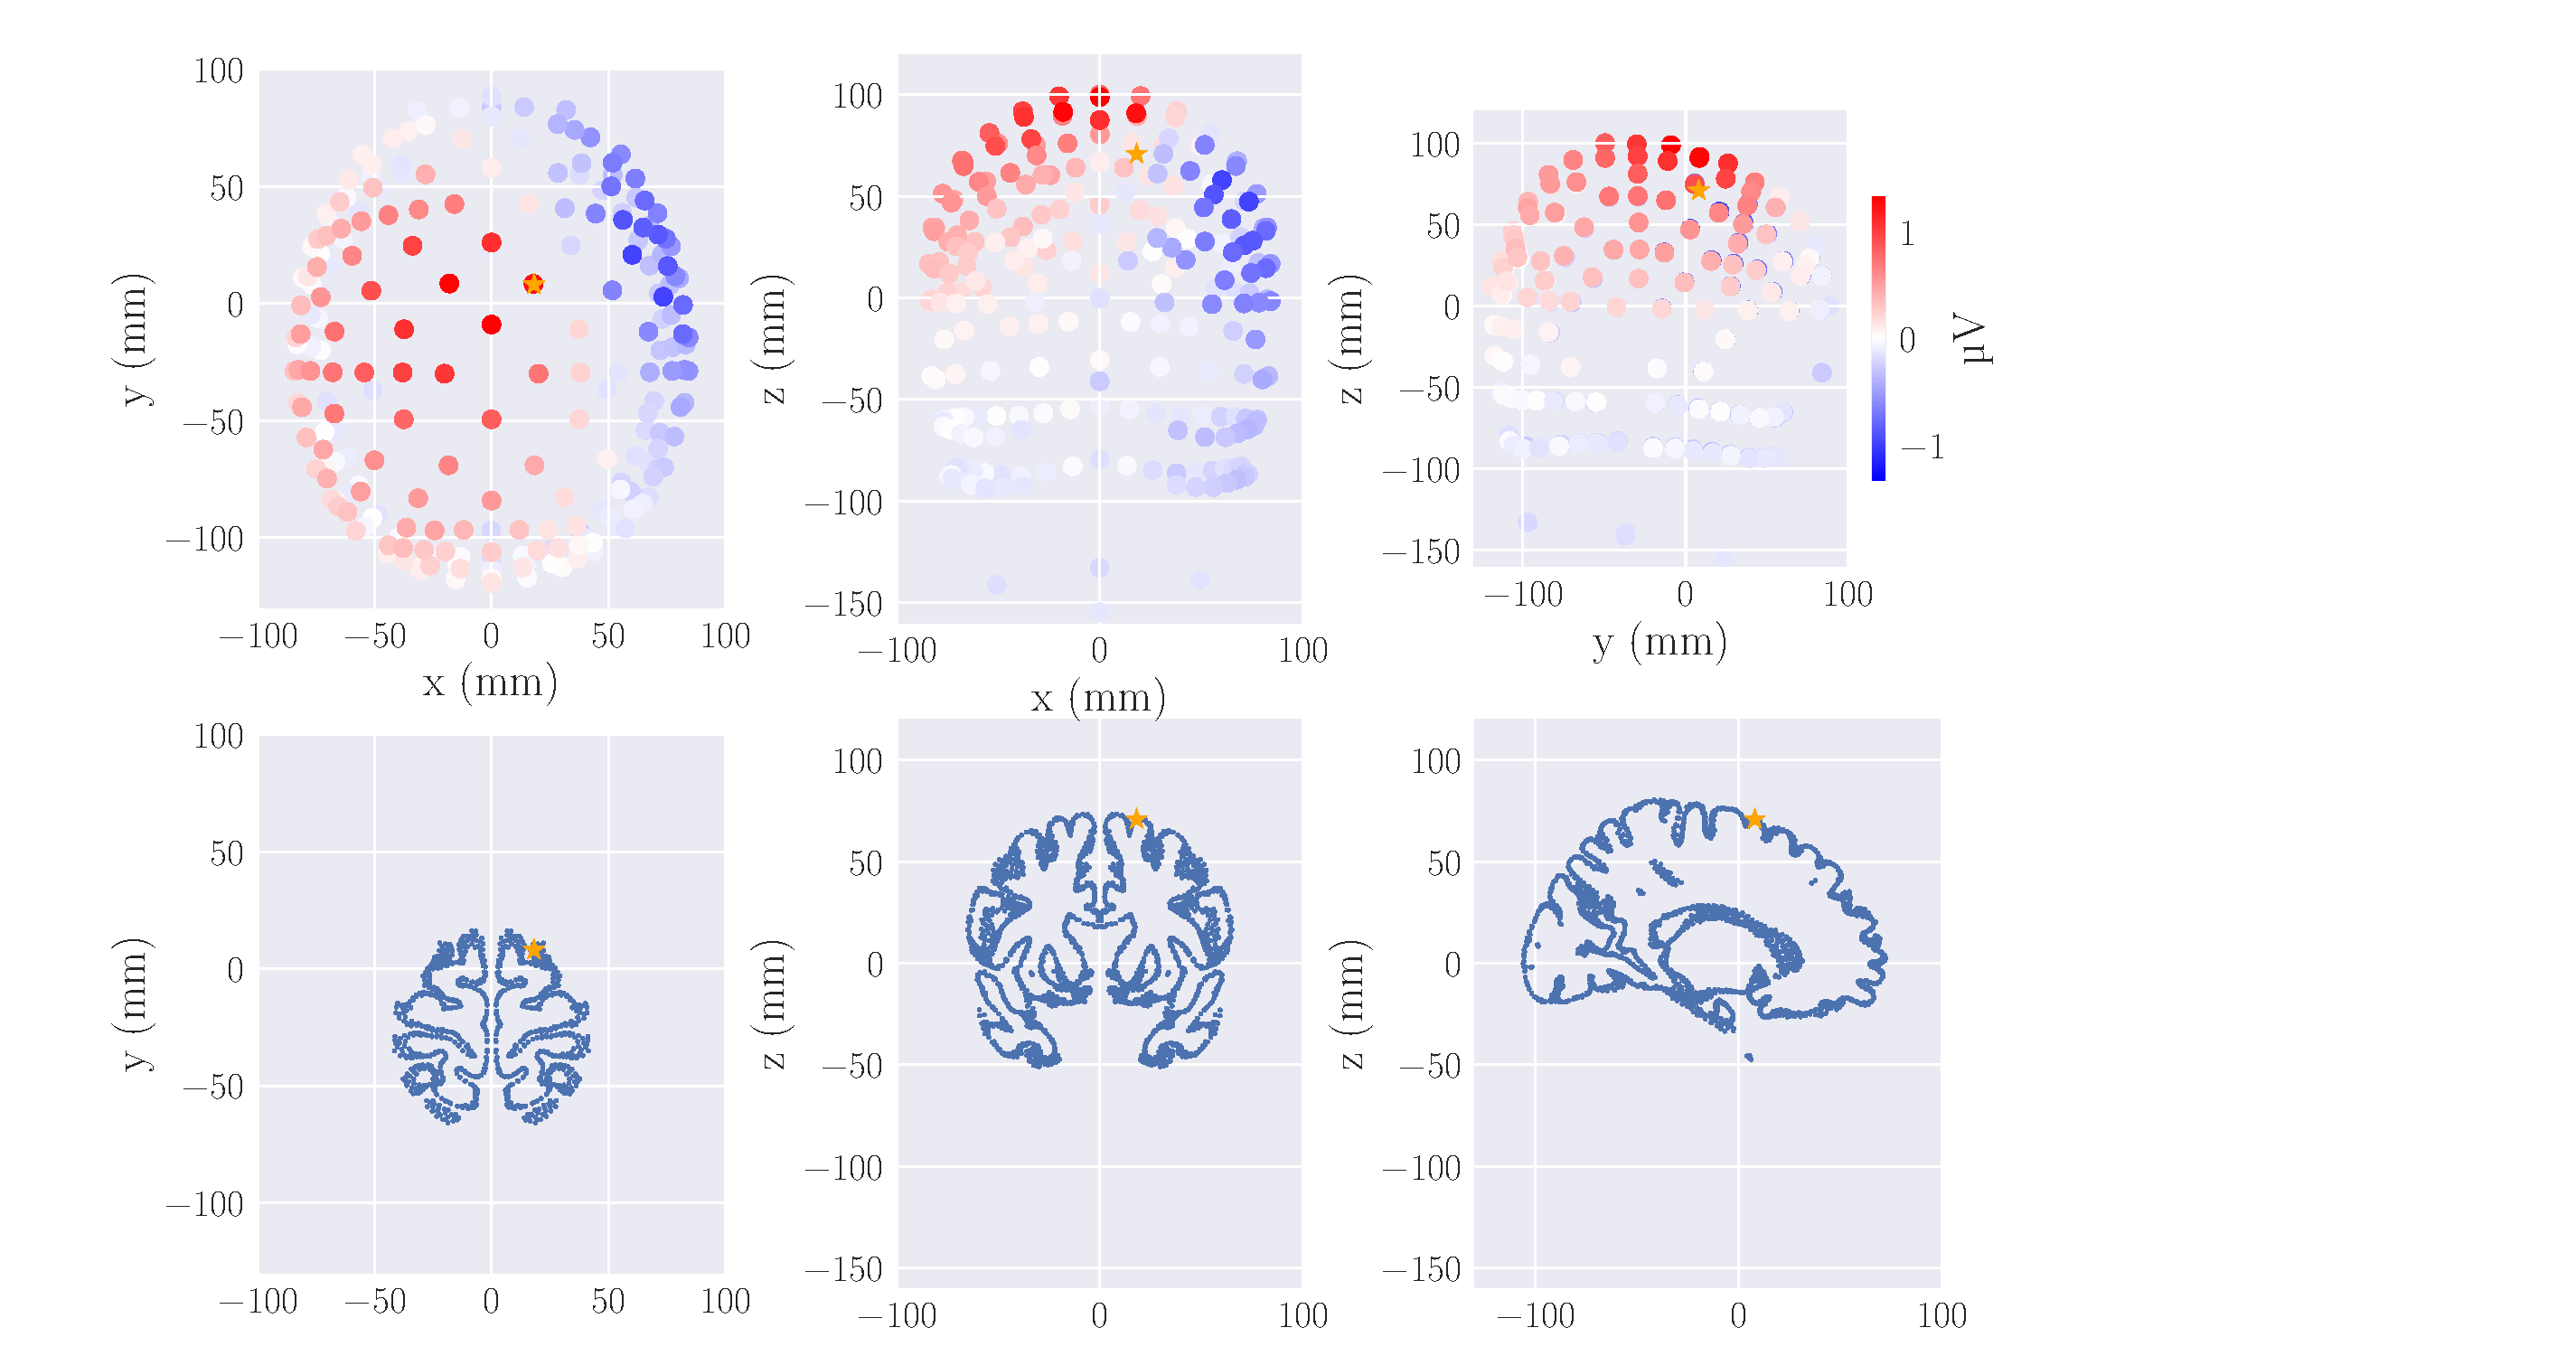
\includegraphics[width=\linewidth]{figures/simple_example.pdf}
    \caption{EEG for a sample containing one single current dipole source at a random position within the celebral cortex. As for all samples within the data set, 10 percent of normally distributed noise has been added to the original signal. The EEG measure is seen from both sides (x-, z-plane and y-, z-plane) and above (the x-, y-plane). EEG electrode locations are presented as filled circels, where the color of the fill represents the amplitude of the measured signal for the given electrode. The position of the current dipole moment is marked with a yellow star.}
    \label{fig:eeg_field_1_dipole_example}
\end{figure}

\subsection{Final Dataset}
The final dataset comprises 70 000 rows, where each row corresponds to a single sample or patient. Within the dataset, there are 231 columns representing the features, which denote the EEG measurements recorded at each electrode. Consequently, the dataset has a size of 70 000 x 231. In practice, the data consists of two separete files holding pairs of EEG data and corresponding target data, where x-, y- and z coordinates of different dipole sources is the answer keys.

Figure \ref{fig:eeg_field_1_dipole_example} presents an example of the input EEG data for a single sample, with 10$\%$ noise added. The illustration showcases the EEG results obtained from a sample containing a solitary current dipole source positioned randomly within the cerebral cortex. The dipolar pattern in the figure indicates that the dipole is located within a sulcus. The EEG measure is visualized from multiple perspectives, including the x-z plane, y-z plane, and the x-y plane. The electrode locations are represented by filled circles, with the color of the fill indicating the amplitude of the measured signal at each electrode. The position of the current dipole moment is denoted by a yellow star. As observed from the figure, the EEG signal for this specific sample ranges from -1 to 1 $\mu$V.




% Before being feed to the DiLoc network for training, the data is splitted into train, validation and test parts. The train- and validation data are the batches of the data set that the network uses during training. Out of the 70 000 samples in the final dateset, 50000 is set off to the purpose of train and validation data. Out of these 50000 sampes, randomly selected 80 percent of the rows are put into the training set. The remaining 20 percent operates as the validation set, which is useful in order to prevent the network to overfit during training. The test set which contains the final 20 000 samples will be used after the training prosess for the purpose of testing how well the model generalizes to new, unseen data.
%
% Prior to being fed into the DiLoc network for training, the dataset was splittied into distinct segments: the train, validation, and test sets. This partitioning is vital for assessing and optimizing the network's performance. Among the 70 000 samples in the final dataset, 50 000 samples are designated for the train and validation data. To ensure a representative and unbiased allocation, 80 percent of these 50 000 samples are randomly assigned to the training set. This training set serves as the core data that the network utilizes during the training process. The remaining 20 percent of the 50 000 samples form the validation set. This set plays the role in preventing overfitting, the phenomenon where the network becomes excessively attuned to the training data and consequently performs poorly on new data. By independently evaluating the model's performance on the validation set throughout training, we can fine-tune the network's parameters to achieve better generalization to unseen data. Once the network completes its training process, the test set comes into play. Comprising 20 000 samples, the test set serves as the benchmark for assessing the model's ability to generalize and make accurate predictions on new data instances. By adhering to this rigorous train-validation-test data partitioning, we ensure a robust evaluation of the DiLoc model's performance and its capacity to effectively handle real-world scenarios with previously unseen data.



\end{document}